%%%%%%%%%%%%%%%%%%%%%%%%%%%%%%%%%%%%%%%%%
% Beamer Presentation
% LaTeX Template
% Version 1.0 (10/11/12)
%
% This template has been downloaded from:
% http://www.LaTeXTemplates.com
%
% License:
% CC BY-NC-SA 3.0 (http://creativecommons.org/licenses/by-nc-sa/3.0/)
%
%%%%%%%%%%%%%%%%%%%%%%%%%%%%%%%%%%%%%%%%%

%----------------------------------------------------------------------------------------
%	PACKAGES AND THEMES
%----------------------------------------------------------------------------------------

\documentclass{beamer}

\mode<presentation> {

% The Beamer class comes with a number of default slide themes
% which change the colors and layouts of slides. Below this is a list
% of all the themes, uncomment each in turn to see what they look like.

%\usetheme{default}
%\usetheme{AnnArbor}
%\usetheme{Antibes}
%\usetheme{Bergen}
%\usetheme{Berkeley}
%\usetheme{Berlin}
%\usetheme{Boadilla}
%\usetheme{CambridgeUS}
%\usetheme{Copenhagen}
%\usetheme{Darmstadt}
%\usetheme{Dresden}
%\usetheme{Frankfurt}
%\usetheme{Goettingen}
%\usetheme{Hannover}
%\usetheme{Ilmenau}
%\usetheme{JuanLesPins}
%\usetheme{Luebeck}
\usetheme{Madrid}
%\usetheme{Malmoe}
%\usetheme{Marburg}
%\usetheme{Montpellier}
%\usetheme{PaloAlto}
%\usetheme{Pittsburgh}
%\usetheme{Rochester}
%\usetheme{Singapore}
%\usetheme{Szeged}
%\usetheme{Warsaw}

% As well as themes, the Beamer class has a number of color themes
% for any slide theme. Uncomment each of these in turn to see how it
% changes the colors of your current slide theme.

%\usecolortheme{albatross}
%\usecolortheme{beaver}
%\usecolortheme{beetle}
%\usecolortheme{crane}
%\usecolortheme{dolphin}
%\usecolortheme{dove}
%\usecolortheme{fly}
%\usecolortheme{lily}
%\usecolortheme{orchid}
%\usecolortheme{rose}
%\usecolortheme{seagull}
%\usecolortheme{seahorse}
%\usecolortheme{whale}
%\usecolortheme{wolverine}

%\setbeamertemplate{footline} % To remove the footer line in all slides uncomment this line
%\setbeamertemplate{footline}[page number] % To replace the footer line in all slides with a simple slide count uncomment this line

%\setbeamertemplate{navigation symbols}{} % To remove the navigation symbols from the bottom of all slides uncomment this line
}

\usepackage{graphicx} % Allows including images
\usepackage[absolute, overlay]{textpos}
\usepackage{booktabs} % Allows the use of \toprule, \midrule and \bottomrule in tables
\usepackage{tikz}
\usepackage{caption}
\usetikzlibrary{positioning,calc,backgrounds,shapes}

\usepackage[labelformat=empty]{caption}
\captionsetup{compatibility=false}
\theoremstyle{definition}
\newtheorem{my_example}[theorem]{Exemplu}


\tikzset{My Arrow Style/.style={single arrow, fill=red!30, anchor=base, align=center,text width=4cm}}
\newcommand{\arrowthis}[2][]{\tikz[baseline] \node [My Arrow Style,#1] {#2};}


\tikzset{My Speech Style/.style={ellipse callout, fill=red!50, anchor=base, align=center,text width=2.8cm}}
\newcommand{\speechthis}[2][]{
    \tikz[baseline]{\node[My Speech Style, #1]{#2};}
}%

\newcommand{\source}[1]{\begin{textblock*}{4cm}(8.7cm,8.2cm)
        \begin{beamercolorbox}[ht=0.5cm,right]{framesource}
        \usebeamerfont{framesource}\usebeamercolor[fg]{framesource} Source: {#1}
        \end{beamercolorbox}
    \end{textblock*}
}
%----------------------------------------------------------------------------------------
%	TITLE PAGE
%----------------------------------------------------------------------------------------

\title[Universitatea din Bucure\c{s}ti]{Aplica\c{t}ii ale Schemelor de Partajare a Secretelor}

% The short title appears at the bottom of every slide, the full title is only on the title page
%An Immediate Multi-Party Generalization of ID-NIKE from Constrained PRF
\author[Drago\c{s} Alin Rotaru]{Drago\c{s} Alin Rotaru} % Your name
\institute[UniBuc] % Your institution as it will appear on the bottom of every slide, may be shorthand to save space
{
Universitatea din Bucure\c{s}ti\\ % Your institution for the title page
% \medskip
% \textit{ruxandra.olimid@fmi.unibuc.ro, r.dragos0@gmail.com} % Your email address
}
\date{9 februarie, 2015} % Date, can be changed to a custom date

\begin{document}

\begin{frame}
\titlepage % Print the title page as the first slide
\end{frame}


%----------------------------------------------------------------------------------------
%	PRESENTATION SLIDES
%----------------------------------------------------------------------------------------

%------------------------------------------------

\AtBeginSection[]
{
  \begin{frame}<beamer>
    \frametitle{Cuprins pentru sec\c{t}iunea \thesection}
    \tableofcontents[currentsection]
  \end{frame}
}

\section{Overview} % Sections can be created in order to organize your presentation into discrete blocks, all sections and subsections are automatically printed in the table of contents as an overview of the talk
%------------------------------------------------

\subsection{Motiva\c{t}ie}
\begin{frame}
    \frametitle{Motiva\c{t}ie: scheme de partajare} % Table of contents slide, comment this block out to remove it
    \only<1-2>{
        \begin{textblock*}{4cm}(3cm, 3cm)
        \begin{figure}
            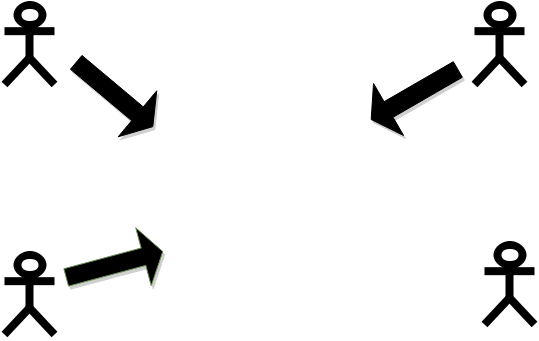
\includegraphics[width=7cm,height=7cm,keepaspectratio]{img/motivation/key1.png}
        \end{figure}
        \end{textblock*}
    }
    \only<2> {
        \begin{textblock*}{4cm}(4.5cm, 4cm)
        \begin{figure}
            
\includegraphics[width=2cm,height=2cm,keepaspectratio]{img/motivation/Lock.png}
        \end{figure}
        \end{textblock*}
    }
    \only<3-> {
        \begin{textblock*}{4cm}(3cm, 3cm)
        \begin{figure}
            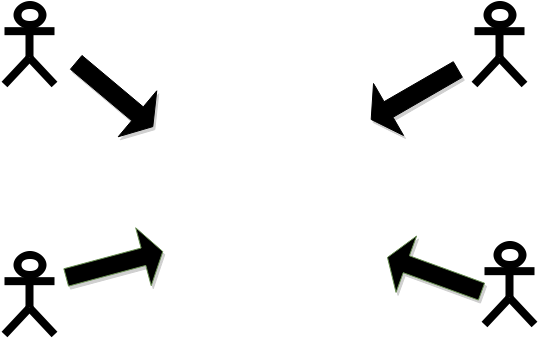
\includegraphics[width=7cm,height=7cm,keepaspectratio]{img/motivation/all_in.png}
        \end{figure}
        \end{textblock*}

        \begin{textblock*}{4cm}(4.5cm, 4cm)
        \begin{figure}
            
\includegraphics[width=2cm,height=2cm,keepaspectratio]{img/motivation/key-128.png}
        \end{figure}
        \end{textblock*}
    }
\end{frame}

\begin{frame}
    \frametitle{Motiva\c{t}ie: sisteme de stocare} 
    \only<1-2> {

        \begin{textblock*}{2cm}(1cm, 4.7cm)
        \begin{figure}
            
\includegraphics[width=2cm,height=2cm,keepaspectratio]{img/motivation/boy-128.png}
        \end{figure}
        \end{textblock*}
    }
    \only<2-2> {

        \begin{textblock*}{4cm}(4cm, 2cm)
        \begin{figure}
            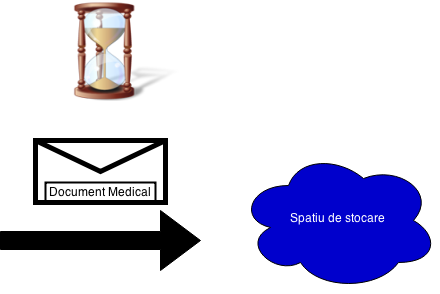
\includegraphics[width=7cm,height=7cm,keepaspectratio]{img/motivation/storage-system.png}
        \end{figure}
        \end{textblock*}
    }
    \only<3-> {

        \begin{textblock*}{2cm}(1cm, 4.7cm)
        \begin{figure}
            
\includegraphics[width=2cm,height=2cm,keepaspectratio]{img/motivation/old-128.png}
        \end{figure}
        \end{textblock*}
    }
    \only<3-> {

        \begin{textblock*}{4cm}(4cm, 2cm)
        \begin{figure}
            
\includegraphics[width=7cm,height=7cm,keepaspectratio]{img/motivation/after_system.png}
        \end{figure}
        \end{textblock*}
    }
\end{frame}

%------------------------------------------------
\section{Scheme de partajare}

\begin{frame}
    \frametitle{Schema Shamir - intui\c{t}ie}
    \only<1-2> {
        \begin{textblock*}{12cm}(1cm,1cm)
            \begin{itemize}
                \item $k$ puncte distincte \^{i}n plan definesc o curb\u{a} polinomial\u{a} unic\u{a} av\^{a}nd grad $k - 1$
                \item Mai pu\c{t}in de $k$ puncte nu pot reconstitui polinomul original
            \end{itemize}
        \end{textblock*}
    }
    \only<2-> {
        \begin{textblock*}{4cm}(4cm, 4.5cm)
        \begin{figure}
            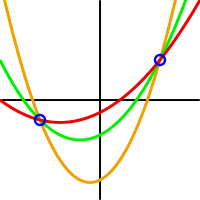
\includegraphics[width=3.5cm,height=2.7cm,keepaspectratio]{img/shamir/shamir.png}
            \caption{"3 polynomials of degree 2 through 2 points" by Vlsergey}
        \end{figure}
        \end{textblock*}
     }
\end{frame}

\subsection{Schema Shamir}
\begin{frame}
    \frametitle{Schema Shamir}
    \begin{itemize}
        \item Secret $\mathcal{S}$
        \pause
        \item Schema $(k,n)$ majoritar\u{a}
        \pause
        \item Oricare $k$ participan\c{t}i din cei $n$ pot reconstitui $\mathcal{S}$
        \pause
        \item Mai pu\c{t}in de $k$ participan\c{t}i nu ob\c{t}in nici o informa\c{t}ie despre $\mathcal{S}$
        \pause
        \item Se alege un polinom $f$ de grad $k - 1$ av\^{a}nd coeficien\c{t}i aleatori, termenul liber fiind $\mathcal{S}$
        \pause
        \item Participantul $P_i$ primeste $f(i)$, $i = \{1, 2, ...n\}$
        \pause
        \item Dup\u{a} reconstituire secretul $\mathcal{S}$ se afl\u{a} \^{i}n $f(0)$.
    \end{itemize}
\end{frame}

\begin{frame}
    \frametitle{Schema Shamir}
    \only<1> {
        \begin{my_example}
           Se consider\u{a} 8 participan\c{t}i, unde oricare $4$ pot reconstitui secretul $\mathcal{S}$.
           Fie polinomul $f(x) = a_3x ^ 3 + a_2x ^ 2 + a_1x + S$, $a_i \leftarrow^R Z_q$, $a_i$ ale\c{s}i \^{i}n mod aleator din $Z_q$.
        \end{my_example}
    }
    \only<2> {
     \begin{textblock*}{4cm}(3cm, 1.5cm)
        \begin{figure}
            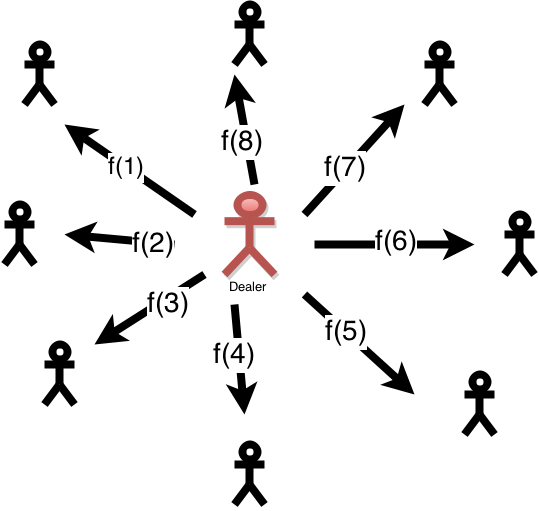
\includegraphics[width=7cm,height=7cm,keepaspectratio]{img/shamir/shamir-split.png}
       \end{figure}
        \end{textblock*}
 
    }
\end{frame}

\subsection{Schema unanim\u{a} XOR}
\begin{frame}
    \frametitle{Schema unanim\u{a} XOR}
    \begin{itemize}
        \item Schema majoritar\u{a} $(n,n)$.
        \pause
        \item $n-1$ participan\c{t}i primesc numere aleatoare: $s_1, s_2, \dots s_{n-1}$.
        \pause
        \item Cel de-al $n$-lea participant prime\c{s}te $S \oplus s_1 \oplus s_2 \oplus \dots \oplus s_{n-1}$.
        \pause
        \item Reconstruc\c{t}ia: $\mathcal{S} = s_1 \oplus s_2 \oplus \dots \oplus s_n$.
    \end{itemize}
\end{frame}

\subsection{Schema Ito, Saito \c{s}i Nishizeki}
\begin{frame}
    \frametitle{Schema Ito, Saito \c{s}i Nishizeki}

    \only<1-> {
    \begin{itemize}
        \item Schema Shamir e insuficient\u{a} pentru a realiza partajarea lui $\mathcal{S}$ unui grup oarecare de participan\c{t}i.
    \end{itemize}
    }
    \only<2-> {
        \begin{textblock*}{4cm}(3.5cm, 5cm)
            \begin{figure}
                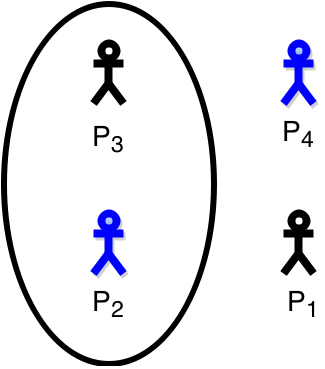
\includegraphics[width=3.5cm,height=3.5cm,keepaspectratio]{img/shamir/Ito.png}
           \end{figure}
        \end{textblock*}
    }
    \only<2-> {

        \begin{textblock*}{4cm}(8cm, 6cm)
            {$\mathcal{S}$ poate fi reconstruit doar din $\{P_2, P_3\}$ sau $\{P_2, P_4\}$}
        \end{textblock*}  
    }
\end{frame}

%------------------------------------------------
\section{Sisteme de stocare}

\subsection{RAID}
\begin{frame}
    \frametitle{Asigurarea disponibilit\u{a}\c{t}ii cu ajutorul sistemelor RAID}
    \begin{itemize}
        \item RAID (Redundant Array of Independent Disks) combin\u{a} 2 concepte ortgonale:
        \pause
            \begin{itemize}
                \item Data striping
                \pause
                \item Redundan\c{t}a datelor 
            \end{itemize}
        \pause
        \item Datele sunt distribuite \^{i}n moduri diferite denumite niveluri RAID.
    \end{itemize}
\end{frame}
\begin{frame}
    \frametitle{Nivelul 0 Raid - Data Striping}
    \begin{textblock*}{4cm}(3cm, 3cm)
        \begin{figure}
            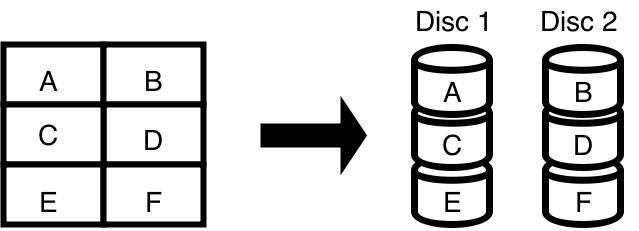
\includegraphics[width=7cm,height=7cm,keepaspectratio]{img/raid/raid0.png}
       \end{figure}
    \end{textblock*}  
\end{frame}

\begin{frame}
    \frametitle{Nivelul 1 Raid - Redundan\c{t}a datelor}
    \begin{textblock*}{4cm}(4cm, 2cm)
        \begin{figure}
            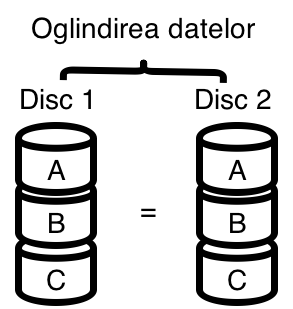
\includegraphics[width=4cm,height=4cm,keepaspectratio]{img/raid/raid1.png}

            \caption{}
       \end{figure}
    \end{textblock*}  
\end{frame}

\begin{frame}
    \frametitle{Sisteme securizate de stocare de lung\u{a} durat\u{a}}
    \begin{itemize}
        \item Securitatea este asigurat\u{a} cu ajutorul schemelor de partajare.
        \pause
        \item Disponibilitatea cu nivele RAID sau scheme de partajare. 
    \end{itemize}
\end{frame}


\subsection{PASIS}

\begin{frame}
    \frametitle{PASIS (2000)}
    \only<1-2> {
        \begin{itemize}
            \item Informa\c{t}ia este partajat\u{a} cu ajutorul agen\c{t}ilor PASIS folosind Schema Shamir.
            \pause
            \item Componentele (share-uri) rezultate in urma partaj\u{a}rii sunt distribuite apoi nodurilor existente \^{i}n re\c{t}ea.
        \end{itemize}
    }
    \only<3-> {
         \begin{textblock*}{4cm}(3cm, 2cm)
            \begin{figure}
                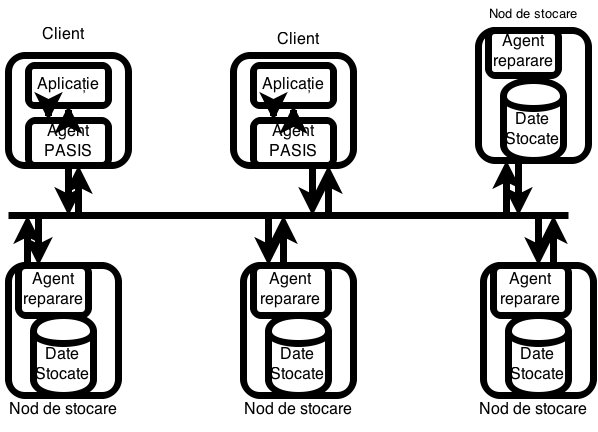
\includegraphics[width=7cm,height=7cm,keepaspectratio]{img/raid/PASIS.png}
           \end{figure}
        \end{textblock*}
    }
\end{frame}

\section{Alouneh et al.}
\begin{frame}
    \frametitle{Alouneh et al. (2013)}
    \begin{itemize}
        \item Informa\c{t}ia este partajat\u{a} cu ajutorul unei aplica\c{t}ii la nivelul clientului folosind o versiune modificat\u{a} a schemei Shamir.
        \pause
        \item Coeficien\c{t}ii polinomului $f$ nu mai sunt ale\c{s}i aleator ci sunt lua\c{t}i direct din fisierul partajat in maniera secvential\u{a}.
        \pause
        \item Nodul cu indexul $i$ prime\c{s}te valoarea polinomului $f(i)$.
    \end{itemize} 
    \pause
    \begin{my_example}
        Fie un fi\c{s}ier $File$ avand octe\c{t}ii: $10$ $15$ \^{i}n aceast\u{a} ordine.

        Polinomul dup\u{a} care se realizeaz\u{a} partajarea este $f(x) = 10 + 15x$.
        Nodul $i$ prime\c{s}te valoarea $f(i)$
    \end{my_example}
\end{frame}
\begin{frame}
    \frametitle{Alouneh et al. (2013): partajare + reconstruc\c{t}ie}
     \begin{textblock*}{4cm}(3cm, 1cm)
        \begin{figure}
            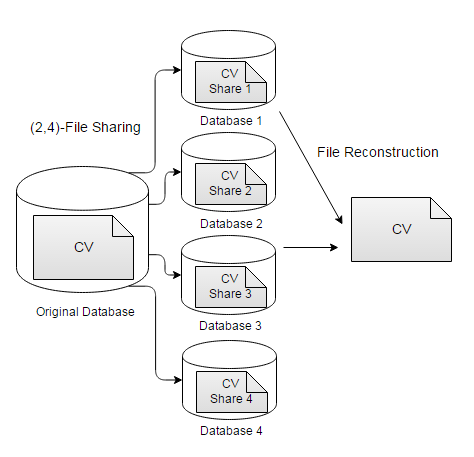
\includegraphics[width=7cm,height=7cm,keepaspectratio]{img/results/sharing.png}
       \end{figure}
    \end{textblock*}
\end{frame}

\section{Rezultate personale}
\begin{frame}
    \frametitle{Alouneh et al. (2013) - atacuri}
    \only<1-2> {
        \begin{itemize}
            \item Construirea polinomului este determinist\u{a}!
            \pause
            \item Componentele rezultate vor fi acelea\c{s}i pentru fi\c{s}iere identice partajate.
        \end{itemize}
    }
    \only<3-> {
        Consider\^{a}nd c\u{a} dealerul $\mathcal{D}$ nu schimb\u{a} numerotoarea nodurilor la diferite distribu\c{t}ii:
        \begin{itemize}
            \item Compararea \^{i}ntre 2 tipuri de fi\c{s}iere partajate pe acela\c{s}i nod este fezabil\u{a}
            \pause
            \item Detectarea fi\c{s}ierelor av\^{a}nd con\c{t}inut similar sau diferit
            \pause
            \item Detectarea unui pattern repetitiv dintr-un fi\c{s}ier
        \end{itemize}
    }
\end{frame}

\subsection{Detectarea tipului de fi\c{s}ier partajat}
\begin{frame}
    \frametitle{Alouneh et al. (2013) - determinarea tipului de fi\c{s}ier partajat}
    Prin ob\c{t}inerea informatiilor dintr-un singur nod, se poate constata tipul de fisier partajat ini\c{t}ial:
    %-----------------------------------------------------
    \only<1-1> {
        \begin{table}[b]
        \bigskip
        \begin{center}
        \caption{Semn\u{a}turi de fi\c{s}iere}\label{tb:margins}
        \label{table:sign}
            \begin{tabular}{ccccc}
            Tip fi\c{s}ier &  \multicolumn{4}{c}{Primii 4 octe\c{t}i}\\ \hline 
            doc &  D0 & CF & 11 & E0\\
            gif & 47 & 49 & 46 & 38 \\
            pdf & 25 & 50 & 44 & 46 \\
            png & 89 & 50 & 4E & 47 \\
            rar & 52 & 61 & 72 & 21 \\
            wav & 52 & 49 & 46 & 46 \\
            zip & 50 & 4B & 03 & 04\\  \hline
            \end{tabular}
        \end{center}
        \bigskip
        \end{table}
    }
    \only<2-2> {
    \begin{table}[t]
        \begin{center}
        \caption{Indicele maxim $i$ a.\^{i}. componentele primului bloc sa fie distincte($k=3$)}\label{tb:margins}
        \label{table:k3}
        \begin{tabular}{cccccccc}
        Tip Fi\c{s}ier & doc & gif & pdf & png & rar & wav & zip \\\hline
          doc & - & 63 & -1 & -1 & -1 & -1 & -1\\
          gif & 63 & - & -1 & -1 & -1 & -1 & -1\\
          pdf & -1 & -1 & - & 164 & -1 & 119 & -1\\
          png & -1 & -1 & 164 & - & 143 & 122 & 129\\
          rar & -1 & -1 & -1 & 143 & - & 143 & -1\\
          wav & -1 & -1 & 119 & 122 & 143 & - & 172\\
          zip & -1 & -1 & -1 & 129 & -1 & 172 & -\\ \hline
        \end{tabular}
        \end{center}
        \bigskip
    \end{table}
    }
\end{frame}

\subsection{Determinarea con\c{t}inutului de fi\c{s}ier}
\begin{frame}
    \frametitle{Alouneh et al. (2013) - determinarea con\c{t}inutului de fi\c{s}ier}
    \only<1-1> {
        \begin{center}
         \begin{textblock*}{4cm}(1cm, 1cm)
            \begin{figure}
                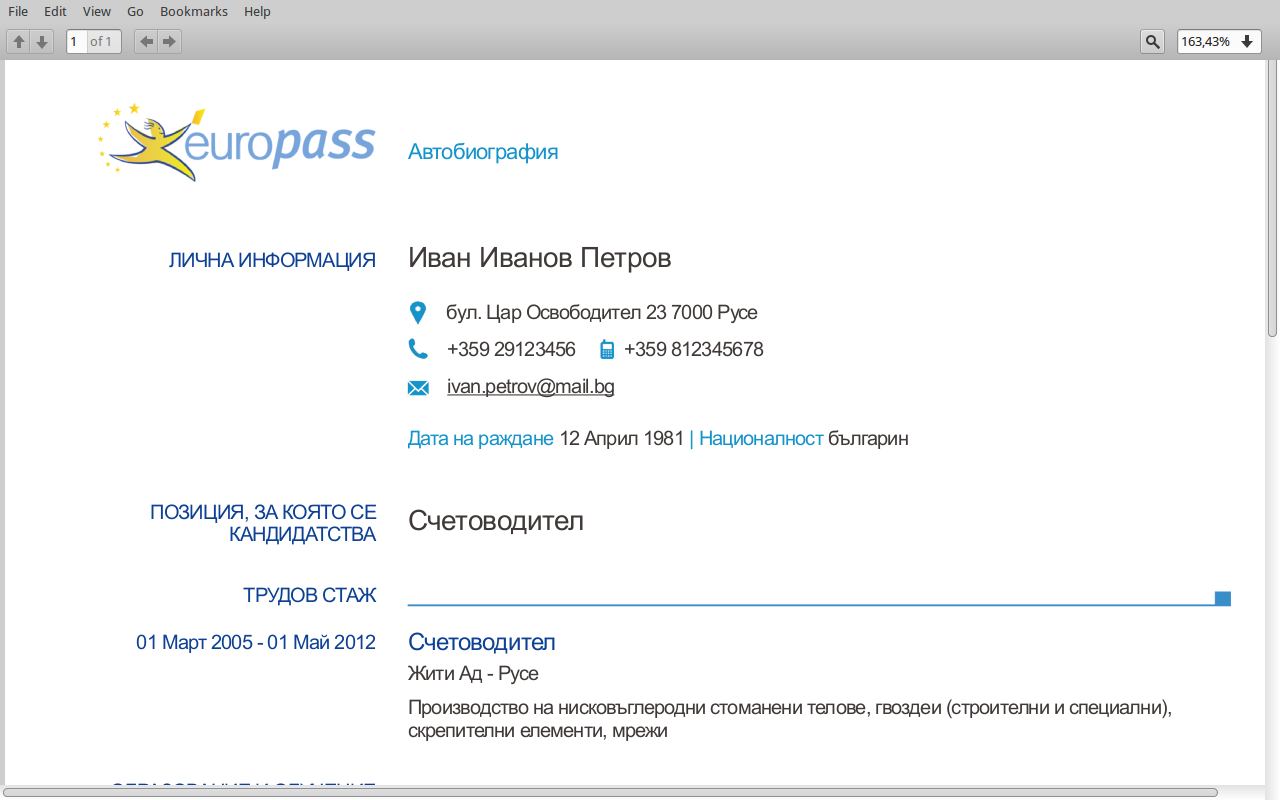
\includegraphics[width=11cm,height=11cm,keepaspectratio]{img/results/CV_BG.png}
                \caption{CV Europass BG}
           \end{figure}
        \end{textblock*} 
        \end{center}
    }
    \only<2-2>{
    \begin{center}
         \begin{textblock*}{4cm}(1cm, 1cm)
            \begin{figure}
                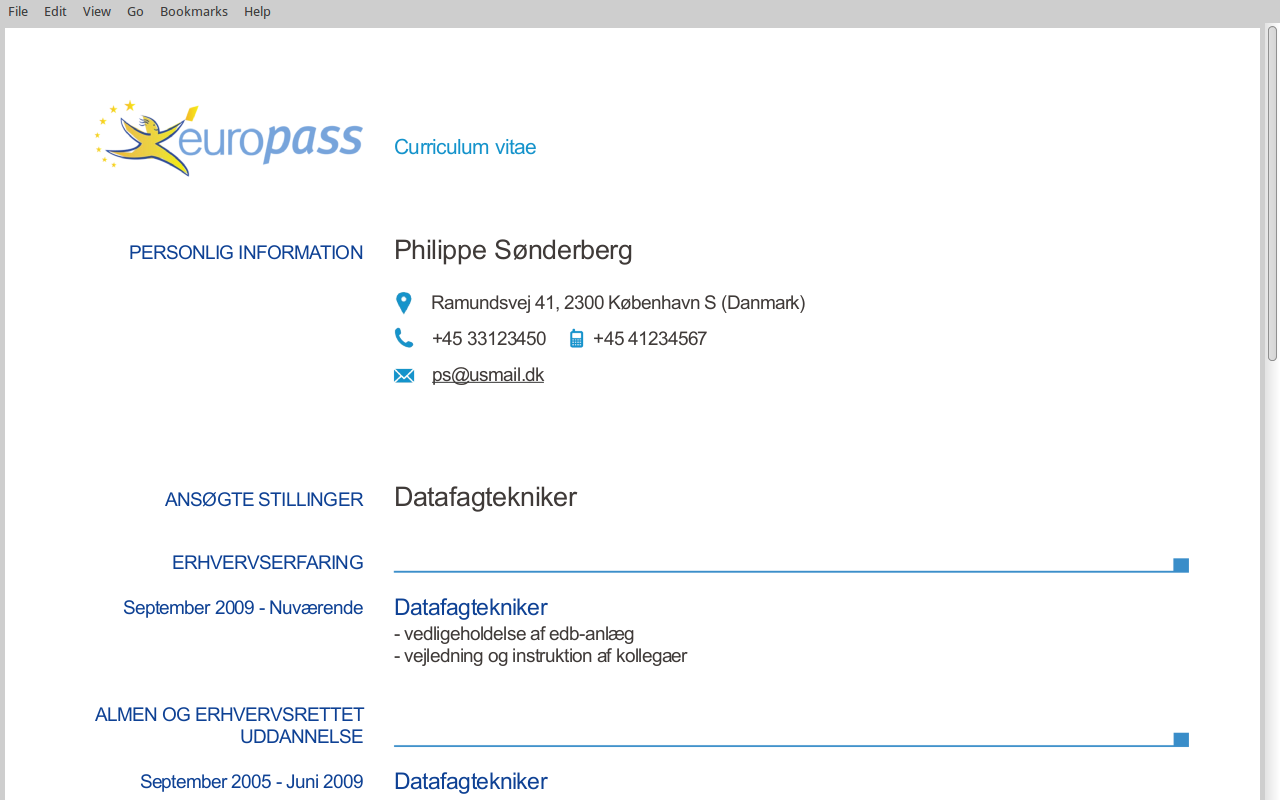
\includegraphics[width=11cm,height=11cm,keepaspectratio]{img/results/CV_DK.png}
                \caption{CV Europass DK}
           \end{figure}
        \end{textblock*} 
        \end{center}
    }
    \only<3-3>{
    \begin{center}
         \begin{textblock*}{4cm}(1cm, 1cm)
            \begin{figure}
                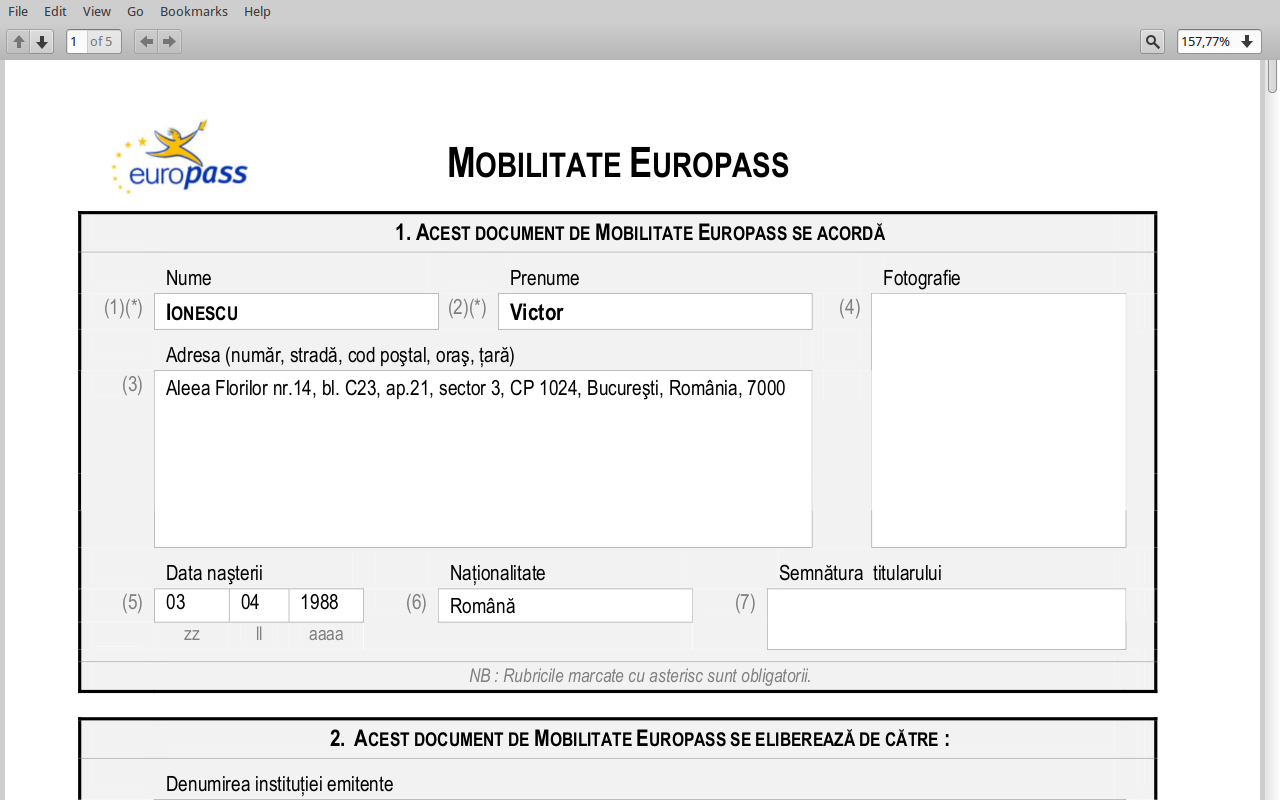
\includegraphics[width=11cm,height=11cm,keepaspectratio]{img/results/RO_MOB.png}
                \caption{Europass Mobility RO}
           \end{figure}
        \end{textblock*} 
        \end{center}
    }
\end{frame}
\begin{frame}
    \frametitle{Alouneh et al. (2013) - determinarea con\c{t}inutului de fi\c{s}ier}
    \begin{textblock*}{4cm}(1cm,2cm)
        Partajarea celor 3 fi\c{s}iere cu schema $(2,4)$. 
    \end{textblock*}

    \only<1> { 
        \begin{textblock*}{4cm}(1cm,5cm)
            Adversarul ob\c{t}ine componentele aflate pe nodul $1$:
        \end{textblock*}
       \begin{textblock*}{4cm}(6cm, 1cm)
            \begin{figure}
                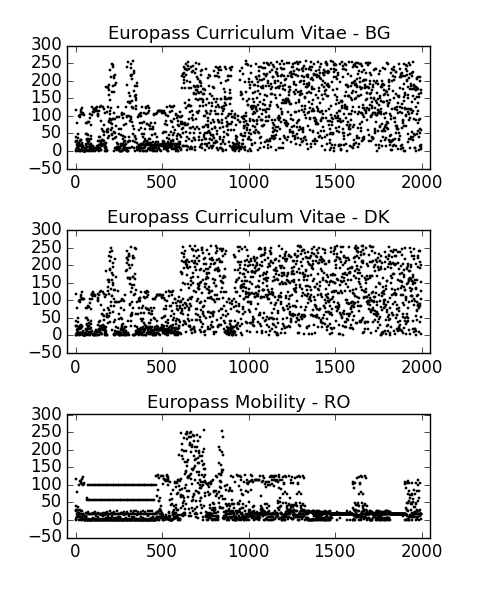
\includegraphics[width=7cm,height=7cm,keepaspectratio]{img/results/db1.png}
           \end{figure}
        \end{textblock*} 
    }
    \only<2> {
    \begin{textblock*}{4cm}(1cm,5cm)
            Adversarul ob\c{t}ine componentele aflate pe nodul $2$:
        \end{textblock*}
       \begin{textblock*}{4cm}(6cm, 1cm)
            \begin{figure}
                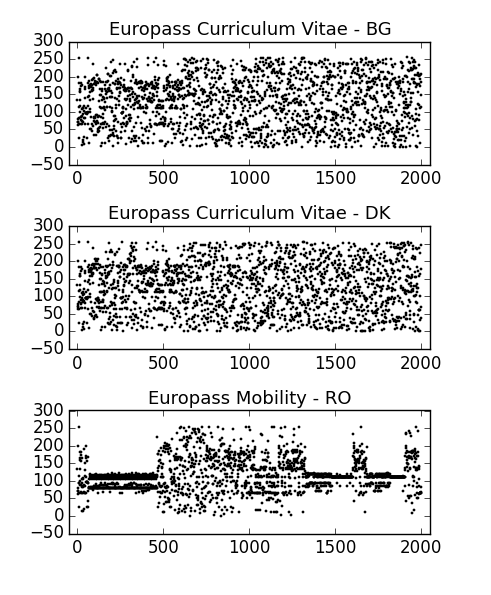
\includegraphics[width=7cm,height=7cm,keepaspectratio]{img/results/db2.png}
           \end{figure}
        \end{textblock*} 
    }
\end{frame}

\subsection{Detectarea unui pattern repetitiv dintr-un fi\c{s}ier}
\begin{frame}

    \frametitle{Alouneh et al. (2013) - determinarea unui pattern \^{i}n fi\c{s}ier}
    \only<1-> {
        \begin{textblock*}{4cm}(7cm, 1cm)
        \begin{figure}
            
\includegraphics[width=4cm,height=4cm,keepaspectratio]{img/results/carouri.png}
        \end{figure}
        \end{textblock*} 
    }
    \only<2-3> {
        \begin{textblock*}{4cm}(1cm, 1cm)
        \begin{figure}
            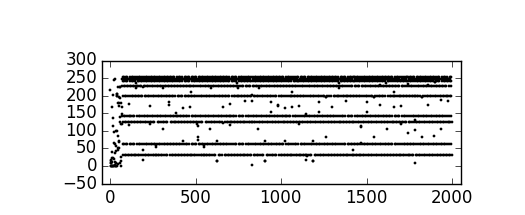
\includegraphics[width=6cm,height=6cm,keepaspectratio]{img/results/carouri_db1.png}
            \caption{Nod 1}
        \end{figure}
        \end{textblock*}
    }
    \only<3-3> {
        \begin{textblock*}{4cm}(1cm, 4.5cm)
        \begin{figure}
            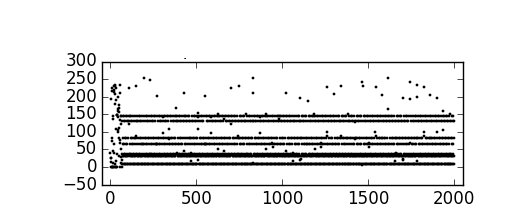
\includegraphics[width=6cm,height=6cm,keepaspectratio]{img/results/carouri_db2.png}
            \caption{Nod 2}
        \end{figure}
        \end{textblock*}
    }
    \only<4-> {
        \begin{textblock*}{4cm}(1cm, 1cm)
        \begin{figure}
            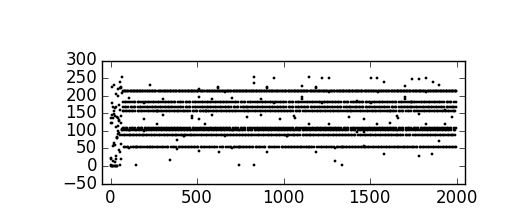
\includegraphics[width=6cm,height=6cm,keepaspectratio]{img/results/carouri_db3.png}
            \caption{Nod 3}
        \end{figure}
        \end{textblock*}
    }
    \only<5-> {
        \begin{textblock*}{4cm}(1cm, 4.5cm)
        \begin{figure}
            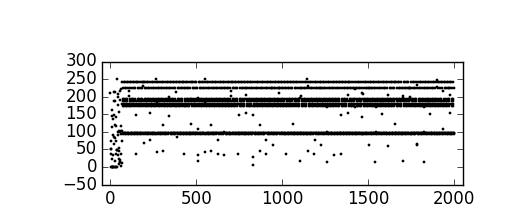
\includegraphics[width=6cm,height=6cm,keepaspectratio]{img/results/carouri_db4.png}
            \caption{Nod 4} 
        \end{figure}
        \end{textblock*}
    }
\end{frame}

\begin{frame}
    \frametitle{Implementare}
    \only<1-2> {
        \begin{itemize}
            \item Python 3.0
            \item Serializarea datelor: Cerealizer
            \item Grafice: Matplotlib
            \pause
            \item Cod surs\u{a}: \href{https://github.com/rdragos/splitting_scheme}{\beamergotobutton{GitHub}}
        \end{itemize}
    }
    \only<3-> {
       \begin{center}
         \begin{textblock*}{4cm}(1cm, 1cm)
            \begin{figure}
                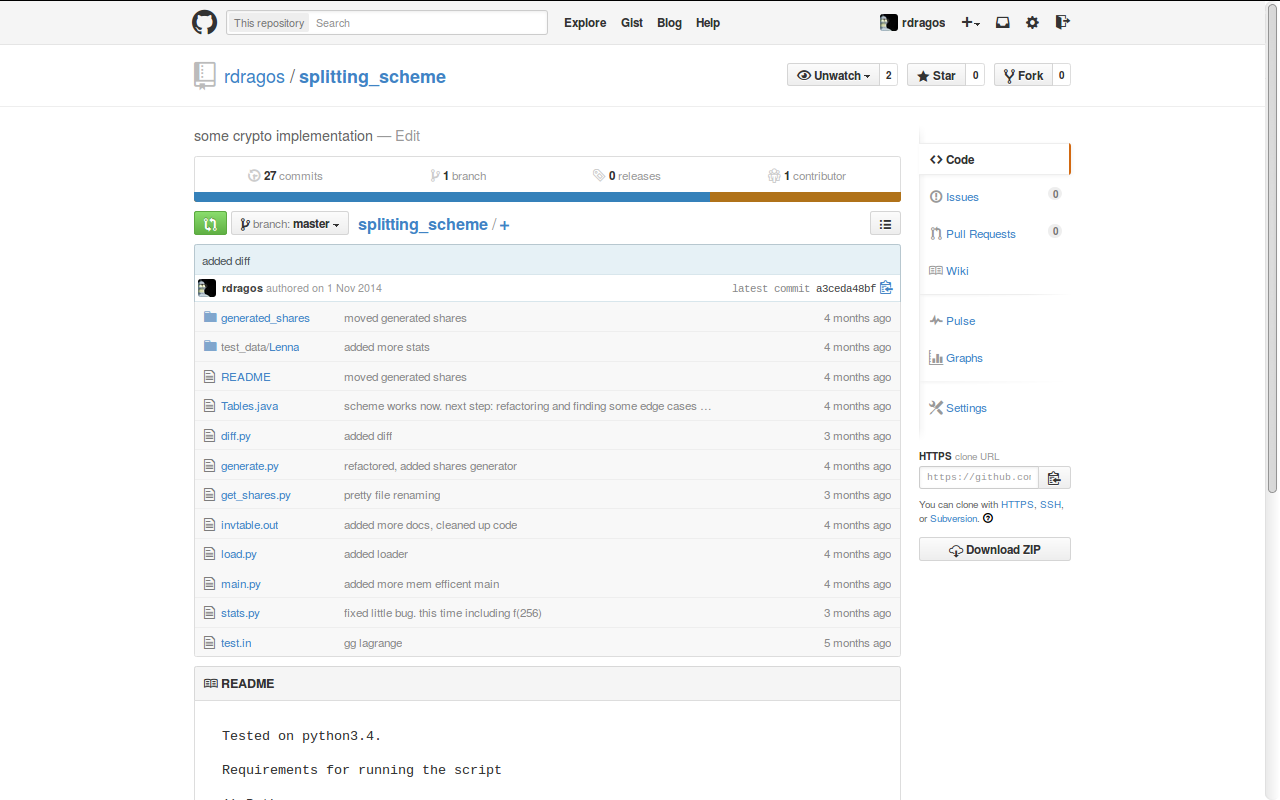
\includegraphics[width=11cm,height=11cm,keepaspectratio]{img/results/github.png}
                \caption{Cod GitHub}
           \end{figure}
        \end{textblock*} 
        \end{center} 
    }
\end{frame}

\begin{frame}
    \frametitle{Prezent}
    \only<1-1> {
        Articolul se afl\u{a} momentan \^{i}n procesul de recenzie la Journal of Control Engineering and Applied Informatics (jurnal indexat ISI,categoria C)
    }
    \only<2-2> {
        \begin{center}
         \begin{textblock*}{4cm}(1cm, 1cm)
            \begin{figure}
                
\includegraphics[width=11cm,height=11cm,keepaspectratio]{img/results/ceai.png}
                \caption{WebSite Jurnal}
           \end{figure}
        \end{textblock*} 
        \end{center} 
    }
\end{frame}
\section{Concluzii}

\begin{frame}
    \frametitle{Concluzii}
    Modificarea unor protocoale criptografice necesit\u{a} demonstra\c{t}ii riguroase!
\end{frame}
\begin{frame}
\Huge{\centerline{Mul\c{t}umesc!}}
\end{frame}

\end{document}